\documentclass[12pt]{amsart}

\addtolength{\hoffset}{-2.25cm}
\addtolength{\textwidth}{4.5cm}
\addtolength{\voffset}{-2.5cm}
\addtolength{\textheight}{5cm}
\setlength{\parskip}{0pt}
\setlength{\parindent}{15pt}
\usepackage{listings}
\usepackage{amsthm}
\usepackage{amsmath}
\usepackage[spanish]{babel}
\usepackage[sort&compress, numbers]{natbib}
\usepackage{amssymb}
\usepackage[utf8]{inputenc}
\usepackage[colorlinks = true, linkcolor = thistle, citecolor = thistle, final]{hyperref}
\usepackage{listings}
\usepackage{ragged2e}
\usepackage{subcaption} 
\usepackage{minted}
\usemintedstyle{borland}
\usepackage{multicol}
\usepackage{listings}
\usepackage{xcolor}
\usepackage{graphicx}
\usepackage[sort&compress, numbers]{natbib}
\usepackage{xcolor}
\usepackage{listings}
\usepackage{ragged2e}
\usepackage{graphicx}
\usepackage[sort&compress, numbers]{natbib}
\usepackage{xcolor}
\usepackage{listings}
\usepackage{ragged2e}
\hypersetup{
    colorlinks=true,
    linkcolor=violet,
    filecolor=violet,     
    urlcolor=violet,
    citecolor=violet,
}
\usepackage{graphicx}
\usepackage[sort&compress, numbers]{natbib}
\usepackage{xcolor}
\usepackage{listings}
\usepackage{ragged2e}

\lstset{style=mystyle}
\usepackage{graphicx}
\usepackage{multicol}
\usepackage{ marvosym }
\newcommand{\ds}{\displaystyle}


\pagestyle{myheadings}

\setlength{\parindent}{0in}
\begin{document}

\pagestyle{empty}



\thispagestyle{empty}

{\scshape Simulación} \hfill {\scshape \Large Tarea 10: Algoritmo genético} \hfill  {\scshape 12/May/2021}
\author{C. María Montemayor Palos}
\maketitle
\hrule
\hrule
\bigskip
\section{Objetivo}
Como objetivo se pretende cambiar la selección de mutación y la selección de los padres para reproducción aplicando la selección de ruleta: cada solución se selecciona como padre con una probabilidad que es linealmente proporcional a su valor de función objetivo y a su factibilidad, combinando los dos a alguna función que parezca conveniente e inversamente proporcional a alguna combinación de factibilidad y objetivo para la mutación.

Se generan instancias con tres distintas reglas:\\
Regla 1: el peso y el valor de cada objeto se generan independientemente con una distribución normal.\\
Regla 2: el valor de cada objeto se generan independientemente con una distribución exponencial y su peso es inversamente correlacionado con el valor, con un ruido normalmente distribuido de baja magnitud.\\
Regla 3: el peso de cada objeto se generan independientemente con una distribución normal y su valor es (positivamente) correlacionado con el cuadrado del peso, con un ruido normalmente distribuido de baja magnitud.\\
Se determina para cada uno de los tres casos a partir de qué tamaño de instancia el algoritmo genético es competitivo con el algoritmo exacto en términos de valor total obtenido por segundo de ejecución y si la inclusión de la selección de ruleta produce una mejora estadísticamente significativa.

\section{Metodología}
Para efectos de la tarea \cite{dra} se utiliza el programa R versión 4.0.4 \cite{R} para Windows. Esta tarea se basa en el problema de la mochila (o mejor conocido en inglés como: knapsack), es un problema clásico de optimización, particularmente de programación entera, donde la tarea consiste en seleccionar un subconjunto de objetos de tal forma que en primer lugar no se exceda la capacidad de la mochila en términos de la suma de los pesos de los objetos incluidos, y en segundo lugar el valor total de los objetos incluidos sea lo máximo posible. Este problema es pseudo-polinomial ya que existe un algoritmo de tabulación que determina la combinación óptima.

\newpage
\section{Código}
Se modifica el código de Schaeffer \cite{codigo} en la sección de las variables correspondiendo \texttt{n} a la capacidad total#, añadiendo \texttt{p0} como población inicial y \texttt{pm} correspondiendo a la población mutada. Esta sección del código es aplicable para las tres reglas.
\renewcommand{\listingscaption}{Código}
\begin{listing}[H]
  \begin{minted}[linenos,mathescape,texcl]{clojure}
n <- 50
pesos <- generador.pesos(n, 15, 80)
valores <- generador.valores(pesos, 10, 500)
capacidad <- round(sum(pesos) * 0.65)
optimo <- knapsack(capacidad, pesos, valores)
init <- 200
p0 <- poblacion.inicial(n, init)
p<- p0
tam <- dim(p)[1]
assert(tam == init)
pm <- sum(runif(tam) < 0.05)
rep <- 50
tmax <- 50
mejorruleta <- double()
  \end{minted}
  \label{codigo1}
\end{listing}

Se genera la probabilidad de mutación y las personas mutadas para la regla 1 aplicando la ruleta.
\renewcommand{\listingscaption}{Código}
\begin{listing}[H]
  \begin{minted}[linenos,mathescape,texcl]{clojure}
  prob.mutacion = NULL
  for (i in 1:tam) {
    prob.mutacion[i] = 1/(obj[i]*(fact[i]+1)*sum(obj*(fact+1)))
  }
  pmutadas<-sample(1:tam, pm, prob = prob.mutacion)
  for (i in pmutadas) {
    p <- rbind(p, mutacion(p[i,], n)) 
  }
  \end{minted}
  \label{codigo1}
\end{listing}

Se generan las reproducciones de los padres y se generan el primer y segundo hijo.
\renewcommand{\listingscaption}{Código}
\begin{listing}[H]
  \begin{minted}[linenos,mathescape,texcl]{clojure}
  prob.reproduccion = NULL
  for (i in 1:tam) {
    prob.reproduccion[i] = obj[i]*(fact[i]+1)/sum(obj*(fact+1))
  }
  for (i in 1:rep) { 
    padres <- sample(1:tam, 2, replace=FALSE, prob = prob.reproduccion)
    hijos <- reproduccion(p[padres[1],], p[padres[2],], n)
    p <- rbind(p, hijos[1:n]) # primer hijo
    p <- rbind(p, hijos[(n+1):(2*n)]) # segundo hijo
  \end{minted}
  \label{codigo1}
\end{listing}

\newpage
Se generan las iteraciones del algoritmo genético sin ruleta, cada objeto puede mutarse con una probabilidad \texttt{pm}.
\renewcommand{\listingscaption}{Código}
\begin{listing}[H]
  \begin{minted}[linenos,mathescape,texcl]{clojure}
 for (iter in 1:tmax) {
  p$obj <- NULL
  p$fact <- NULL
  for (i in 1:tam) { 
    if (runif(1) < pm) {
      p <- rbind(p, mutacion(p[i,], n))
    }
  }
  \end{minted}
  \label{codigo1}
\end{listing}

Código sin ruleta.
\renewcommand{\listingscaption}{Código}
\begin{listing}[H]
  \begin{minted}[linenos,mathescape,texcl]{clojure}
for (i in 1:rep) { 
    padres <- sample(1:tam, 2, replace=FALSE)
    hijos <- reproduccion(p[padres[1],], p[padres[2],], n)
    p <- rbind(p, hijos[1:n]) # primer hijo
    p <- rbind(p, hijos[(n+1):(2*n)]) # segundo hijo
  }
  tam <- dim(p)[1]
  obj <- double()
  fact <- integer()
  for (i in 1:tam) {
    obj <- c(obj, objetivo(p[i,], valores))
    fact <- c(fact, factible(p[i,], pesos, capacidad))
  }
  p <- cbind(p, obj)
  p <- cbind(p, fact)
  mantener <- order(-p[, (n + 2)], -p[, (n + 1)])[1:init]
  p <- p[mantener,]
  tam <- dim(p)[1]
  assert(tam == init)
  factibles <- p[p$fact == TRUE,]
  mejor <- max(factibles$obj)
  mejorsin <- c(mejorsin, mejor)
}
  \end{minted}
  \label{codigo1}
\end{listing}

Modificación del código para la regla 1 en el cual el peso y el valor de cada objeto se genera independientemente con una distribución normal.

\renewcommand{\listingscaption}{Código}
\begin{listing}[H]
  \begin{minted}[linenos,mathescape,texcl]{clojure}
generador.pesos <- function(cuantos, min, max) {
  return(sort(round(normalizar(rnorm(cuantos)) * (max - min) + min)))
}
  \end{minted}
  \label{codigo1}
\end{listing}

\newpage
Modificación del código para la regla 2 en la cual el valor de cada objeto se genera independientemente con una distribución exponencial y su peso es inversamente correlacionado con el valor, con un ruido normalmente distribuido de baja magnitud.

\renewcommand{\listingscaption}{Código}
\begin{listing}[H]
  \begin{minted}[linenos,mathescape,texcl]{clojure}
generador.pesos <- function(valores, min, max) {
  n <- length(valores)
  pesos <- double()
  for (i in 1:n) {
    media <- valores[i]
    desv <- runif(1, max=.1)
    ruido <- rnorm(1, sd=.1)
    pesos <- c(pesos, rnorm(1, (1/media), desv) + ruido)
  }
  pesos <- normalizar(pesos) * (max - min) + min
  return(pesos)
}
  \end{minted}
  \label{codigo1}
\end{listing}

Modificación del código para la regla 3 en la cual el peso de cada objeto se generan independientemente con una distribución normal y su valor correlacionado con el cuadrado del peso, con un ruido normalmente distribuido de baja magnitud.
\renewcommand{\listingscaption}{Código}
\begin{listing}[H]
  \begin{minted}[linenos,mathescape,texcl]{clojure}
generador.valores <- function(pesos, min, max) {
  n <- length(pesos)
  valores <- double()
  for (i in 1:n) {
    media <- pesos[i]
    desv <- runif(1)
    ruido <- rnorm(1, sd=.1)
    valores <- c(valores, rnorm(1, media^2, desv) + ruido)
  }
  valores <- normalizar(valores) * (max - min) + min
  return(valores)
}
  \end{minted}
  \label{codigo1}
\end{listing}

\clearpage
\section{Resultados y discusión}
En las siguientes figuras se presentan los resultados obtenidos de las reglas 1, 2 y 3 respectivamente, correspondiendo la línea verde al valor óptimo, la línea morada a la ejecución del código sin ruleta y a la línea rosa pastel a la ejecución del código con la ruleta.

\begin{figure}[h!]
    \centering
    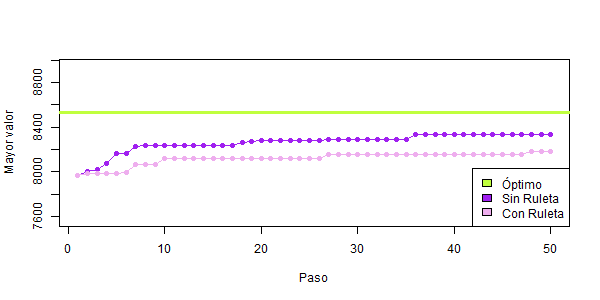
\includegraphics[width=0.5\textwidth]{t10_1.png}
    \caption{Diagrama de ejecución de la regla 1 con ruleta y sin ruleta.}
    \label{fig1}
\end{figure}

\begin{figure}[h!]
    \centering
    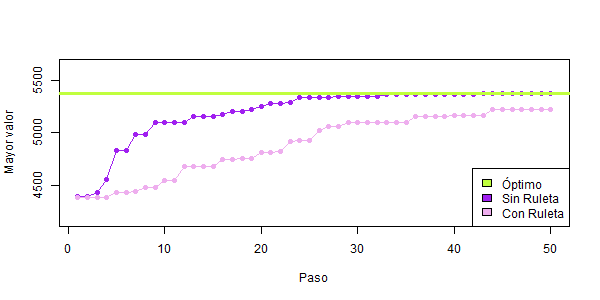
\includegraphics[width=0.5\textwidth]{t10_2.png}
    \caption{Diagrama de ejecución de la regla 2 con ruleta y sin ruleta.}
    \label{fig2}
\end{figure}

\begin{figure}[h!]
    \centering
    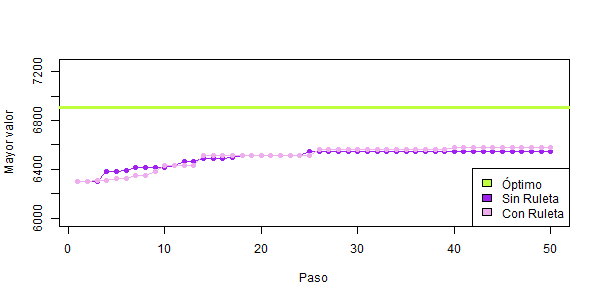
\includegraphics[width=0.5\textwidth]{t10_3.png}
    \caption{Diagrama de ejecución de la regla 3 con ruleta y sin ruleta.}
    \label{fig3}
\end{figure}

\clearpage
De acuerdo a los datos arrojados para cada regla, se comparan los valores obtenidos en la siguiente tabla.

\begin{table}[ht]
    \caption{Fragmento de los datos recopilados del experimento.}
    \label{datos1}
    \centering
    \begin{tabular}{|r|r|r|r|}
       \hline
        Regla&Mejor resultado&Valor óptimo&Porcentaje\\
        \hline
        1&8331 & 8530 & 0.0233 \\
        2&5373 & 5376 & 0.0005 \\
        3&6549 & 6907 & 0.0518 \\
        \hline
    \end{tabular}
\end{table}


\section{Conclusión}
A simple vista se puede deducir por las figuras presentadas que la figura \ref{fig2}, en cuanto a la ejecución del código sin ruleta, fue la más cercana al valor óptimo. Se puede comprobar mediante los datos arrojados observados en la tabla \ref{datos1} que su mejor resultado fue de 5,373 siendo que el valor óptimo fue de 5,376 obtienendo un porcentaje de 0.0005. Comparando los demás valores le sigue la regla 1 (figura \ref{fig1}) resultando como último la regla 3 (figura \ref{fig3}). 

\section{Reto 1}
El primer reto consiste en extender la selección de ruleta a la fase de supervivencia: en vez de quedarse con las mejores soluciones, cada solución tiene una probablidad de entrar a la siguiente generación que es proporcional a su valor de la función objetivo, incorporando el sí o no es factible la solución en cuestión, permitiendo que los $k$ mejores entre las factibles entren siempre (donde $k$ es un parámetro). Se estudia nuevamente el efecto de este cambio en la calidad de la solución en los tres casos.

Modificando el primer código de la regla 1,2 y 3, en la creación de variables se agrega la probabilidad de supervivencia.

\renewcommand{\listingscaption}{Código}
\begin{listing}[H]
  \begin{minted}[linenos,mathescape,texcl]{clojure}
n <- 50
pesos <- generador.pesos(n, 15, 80)
valores <- generador.valores(pesos, 10, 500)
capacidad <- round(sum(pesos) * 0.65)
optimo <- knapsack(capacidad, pesos, valores)
init <- 200
p1 <- poblacion.inicial(n, init)
p<- p1
tam <- dim(p)[1]
assert(tam == init)
pm <- sum(runif(tam) < 0.05)
rep <- 50
tmax <- 50
mejorescon <- double()
prob.supervivencia <- NULL
  \end{minted}
  \label{codigo1}
\end{listing}

\clearpage
En los vectores de factibilidad y objetivos se modifica añadiendo los \texttt{sobrevivientes} para obtener la mejor combinación.

\renewcommand{\listingscaption}{Código}
\begin{listing}[H]
  \begin{minted}[linenos,mathescape,texcl]{clojure}
  p <- cbind(p, obj)
  p <- cbind(p, fact)
  for (i in 1:tam) {
    prob.supervivencia[i] = obj[i]*(fact[i]+1)/sum(obj*(fact+1))
  }
  sobrevivientes<-sample(1:tam,init,prob = prob.supervivencia)
  p <- p[sobrevivientes,]
  tam <- dim(p)[1]
  assert(tam == init)
  factibles <- p[p$fact == TRUE,]
  mejor <- max(factibles$obj)
  mejorruleta <- c(mejorruleta, mejor)
}
  \end{minted}
  \label{codigo1}
\end{listing}

En las siguientes figuras se presentan los resultados obtenidos del reto 1 para las reglas 1, 2 y 3 respectivamente, correspondiendo la línea verde al valor óptimo, la línea morada a la ejecución del código sin ruleta y a la línea rosa pastel a la ejecución del código con la ruleta.

\begin{figure}[h!]
    \centering
    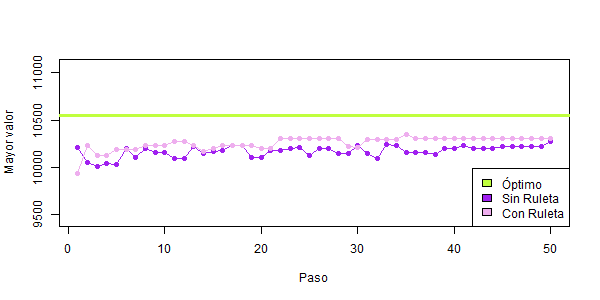
\includegraphics[width=0.5\textwidth]{t10_r1regla1.png}
    \caption{Diagrama de ejecución de la regla 1 con ruleta y sin ruleta.}
    \label{fig4}
\end{figure}

\begin{figure}[h!]
    \centering
    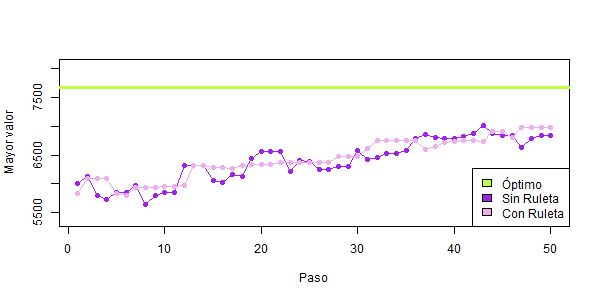
\includegraphics[width=0.5\textwidth]{t10_r1regla2.png}
    \caption{Diagrama de ejecución de la regla 2 con ruleta y sin ruleta.}
    \label{fig5}
\end{figure}

\clearpage
\begin{figure}[h!]
    \centering
    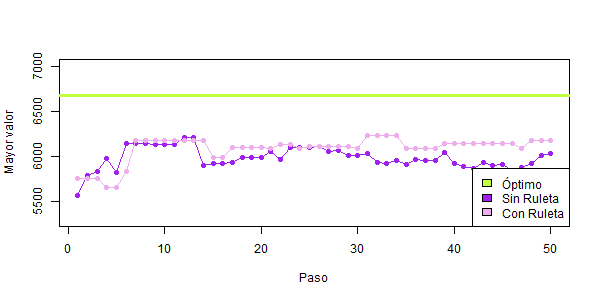
\includegraphics[width=0.5\textwidth]{t10_r1regla3.png}
    \caption{Diagrama de ejecución de la regla 3 con ruleta y sin ruleta.}
    \label{fig6}
\end{figure}


De acuerdo a los datos arrojados para cada regla del reto 1, se comparan los valores obtenidos en la siguiente tabla.

\begin{table}[h!]
    \caption{Comparación de los datos recopilados del experimento.}
    \label{datos2}
    \centering
    \begin{tabular}{|r|r|r|r|}
       \hline
        Regla&Mejor resultado&Valor óptimo&Porcentaje\\
        \hline
        1&10279 & 10553 & 0.0259 \\
        2&6837 & 7676 & 0.1093 \\
        3&6031 & 6682 & 0.0973 \\
        \hline
    \end{tabular}
\end{table}

Como conclusión observando la figura \ref{fig4} tiene valores más cercanos al valor óptimo a comparación de las figuras \ref{fig5} y \ref{fig6}. Comparando los valores del experimento en la tabla \ref{datos2} se aprecia que el mejor resultado es para la regla 1 obteniendo un porcentaje de 0.0259, seguido de la regla 3 con un porcentaje de 0.0973, y por último la regla 2 con un porcentaje de 0.1093.

\clearpage
\bibliography{referencias}
\bibliographystyle{plainnat}


\end{document}